%\subsection{Fase final}
%La recta final del desenvolupament del backend del projecte, s'inicia en el moment en el que s'acaba l'adaptació del mateix amb les noves metodologíes de funcionament.\\ 
%Un cop arribats a aquest estadi, es decideix que el que s'ha de publicar a la \textit{blockchain} no és el hash del consentiment informat, sino el hash d'un document que certifiqui que un usuari determinat, en un moment determinat i amb un codi OTP determinat, ha signat mitjançant l'anterior OTP un consentiment informat amb una empremta digitar determinada.\\
%Per aquest fet, es decidieix modificar la forma amb la que es generen els documents; creant un microservei encarregat d'aquesta tasca.\\
%Aquest nou microservei disposa d'una senzilla API Rest que ens permet enviar les dades necessàries per a que ens torni com a resposta el contingut, codificat en base64, del document desitjat; ja sigui el consentiment informat o bé el coprovant de signatura.\\
%Amb la creació d'aquest microservei independitzem el procés de creació de documents del nucli del projecte, alhora que guanyem una important millora en el temps de creació de documents.\\
%\newline L'esquema resultant del projecte és el següent:\\
%\newline \textit{\textbf{esquema resultant de la plataforma}}\\
%\newline \textit{\textbf{Parlar dels canvis al model de dades + esquema de les taules}}
%Pel que fa al model de dades resultant, hem passat d'un simple parell de taules a la base de dades (figura anterior), a tenir-ne unes cuantes més, a la figura següent es pot veure el model resultant:\\
%\newline \textbf{\textit{model actual}}
\subsection{Model final}
Una vegada decidit el nou rumb que segueix el desenvolupament, cal tenir clares quines son les tasques que manca desenvolupar:
\begin{itemize}
    \item Generar i validar OTP.
    \item Certificar signatura i contingut del consentiment informat.
\end{itemize}
Cal recordar que la capacitat d'enviar SMS ja està integrada dins de la plataforma \textit{Made of Genes}, per tant es pot reutilitzar sense problemes.
\subsubsection{Generació i validació d'OTPs}
Per a la generació de codis OTP (secció \ref{estatArt:signature}), s'ha implementat fil per randa l'algorisme descrit al quart punt de l'especificació\footnote{https://tools.ietf.org/html/rfc6238#section-4}.\\
\newline Seguint amb les directrius de codi que donen la \nameref{arquitectura:back_clean} i \nameref{arquitectura:back_solid}, s'ha encapsulat el codi i modularitzat de tal forma que sigui senzill de llegir i mantenir.
%\begin{itemize}
%\item El primer ragment fa referència a la creació de codis OTP
\begin{listing}[h]
\inputminted[
    firstline=120, 
    lastline=131,
    fontsize=\footnotesize]{php}{resources/src/OTPService.php}
\caption{Mètode de creació de codis OTP}
\label{code:createOTP}
\end{listing}
%\item El segon fragment, a la validació.
\begin{listing}[h]
\inputminted[
    firstline=299, 
    lastline=315,
    fontsize=\footnotesize]{php}{resources/src/OTPService.php}
\caption{Mètode de validació de codis OTP}
\label{code:validateOTP}
\end{listing}
%\end{itemize}
\newline Els fragments de codi que es poden veure sobre aquestes línies, representen cada un dels casos d'ús vistos a la secció \ref{arquitectura:otp} en referència la generació i validació de codis OTP, respectivament.\\
\newline Si es mira el codi detingudament, es pot apreciar que ambdós mètodes tenen pràcticament el mateix comportament, idèntiques crides a funcions.\\
\newline La diferència es troba en el fragment que correspon al procés de validació (Fragment \ref{code:validateOTP}). Aquest executa \textit{n} vegades el procés de generació de codis OTP, sent \textit{n} un enter que oscil·la entre \textit{-TIME\_RANGE} i \textit{TIME\_RANGE}, sent \textit{TIME\_RANGE} una constant definida al codi que actua com a finestra de temps, que permet donar un temps de validesa al codi OTP.\\
\newline Si el codi generat a cada iteració és igual que el codi que s'està evaluant, s'atura l'exeució i el sistema retornarà \textit{true}. En cas contrari, \textit{false}.\\
\newline Els mètodes \textit{oath\_hotp} i \textit{oath\_truncate} es poden trobar a l'annex titulat ``\nameref{appendix:otp}''.

\subsubsection{Certificació de signatura del consentiment informat}
Com s'ha dit a la secció anterior d'aquest mateix capítol (\nameref{desenvolupament:alternatives}), per a la certificació de signatures es farà ús de \textit{blockchain}.\\
Per a una descripció detallada sobre aquesta tecnologia, veure la secció \ref{estatArt:blockchain}.\\
\newline L'objectiu d'aquest punt, és poder donar proves irrefutables de que en un moment donat, un usuari determinat va signar amb un codi OTP concret, un consentiment informat determinat.\\
Per aquest motiu, el projecte es nodreix de la propietat \textit{tamper-proof} (en català immutabilitat) que caracteritza \textit{blockchain}.\\
\newline Un dels motius pels quals s'ha triat aquesta opció en front del certificat digital, és l'existència de serveis que permeten la publicació de \textit{hash} a \textit{blockchain}, permetent al desenvolupador abstraure's de tot el que suposa realitzar una transacció de bitcoin per adderir el \textit{hash} a la cadena de blocs.\\
\clearpage
És el cas d'\textit{OriginStamp}\footnote{\url{https://originstamp.org}}, un servei gratuït que precisament permet publicar \textit{hash} a la \textit{blockchain}, i que dotarà als processos de signatura del no repudi que necessiten.\\
\begin{figure}[h]
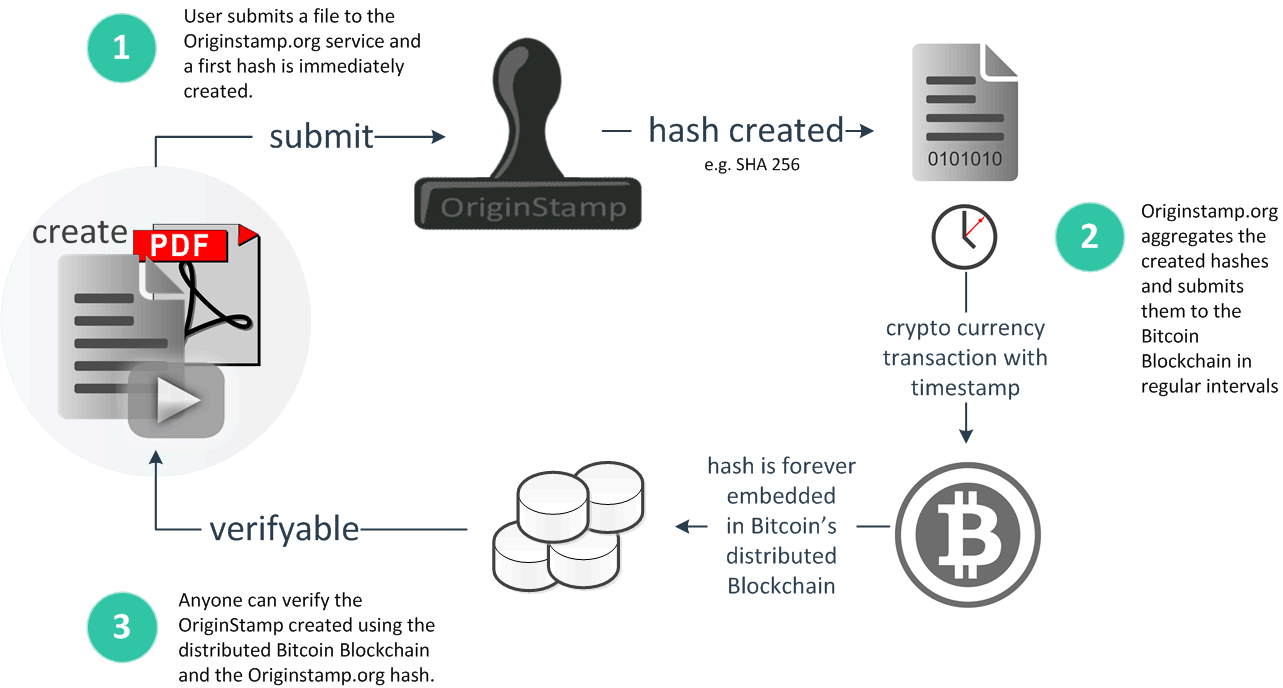
\includegraphics[scale=0.5]{sections/developement/originStamp_workflow.png}
\centering
\caption{OriginStamp}
\label{fig:originStamp}
\end{figure}
\newline La Figura \ref{fig:originStamp}, extreta de la documentació del propi servei, ens mostra el seu funcionament.\\
Tal i com indica l'anterior figura, \textit{OriginStamp} agrega \textit{hash} durant un lapse determinat de temps (24 hores). Un cop passat aquest lapse, afegeix els \textit{hash} que ha acumulat a la \textit{blockchain}, quedant ja per sempre registrats.\\
%\newline Com tot bon servei, ofereix una API amb la qual treballar i integrar els seus serveis al projecte.\\
\newline Continuant amb l'arquitectura general del projecte, aquesta funcionalitat s'ha encapsulat en un servei que permet la re-utilització d'aquest codi en qualsevol punt del projecte.\\
A nivell d'implementació, es tracta de fer crides \textit{HTTP/Post} a la API amb el \textit{hash} en qüestió.\\
\newline A més a més de la \textit{blockchain}, s'ha decidit fer ús d'un servei de segellat de temps (en anglès \textit{timestamping}) per a donar més força a la signatura del consentiment informat.\\
Aquest servei, oferit per FreeTSA\footnote{\url{https://freetsa.org}} permet crear peticions de timestamp (tsq) mitjançant \textit{OpenSSL}.\\
\newline La implementació és similar a la del servei anterior, el servei que encapsula la funcionalitat de \textit{timestamping} fa de pont entre el backend del projecte i el servei de \textit{FreeTSA}.
%A l'annex titulat ``\nameref{appendix:tsa}'' es pot veure la implementació sencera del servei que permet crear els segells de temps sobre els hash dels documents generats.\\
\newline Amb aquests dos serveis fent la mateixa funció, però en serveis que fan servir tecnologies diferents, aconseguim un sistema robust amb doble verificació de signatura, una per part de \textit{blockchain} i l'altre per part de la TSA.\\
Ambdós serveis, a més a més, disposen de mètodes de validació d'existència del \textit{hash}, un afegit amb un valor molt alt de cara el projecte.
\clearpage
\subsubsection{Refactor i millores}
Un cop acabat el desenvolupament global del projecte, s'han aplicat millores al projecte que cal esmentar.\\
Particularment la que fa referència a la creació dels documents.\\
\newline Fins ara, recordem que la creació de documents era responsabilitat del propi \textit{backend} quefeia ús de la llibreria de renderitzat \textit{Twig} i d'una llibreria externa per a la conversió de les plantilles en \textit{HTML} a pdf.\\
\newline Tot i les grans capacitats del tàndem que formen \textit{twig} i la llibreria \textit{wkhtmltopdf}, el punt flac d'aquest duo és la gran latència a l'hora de generar documents pdf.\\
\newline Per aquest motiu, aprofitant la incursió de l'us de serveis externs al projecte, s'ha decidit crear un petit servei,  en forma d'API Rest externa al \textit{backend} del projecte, que permeti la creació de documents de forma dinàmica a partir de plantilles bastant més riques que les emprades amb \textit{twig}, i sobre tot, amb una velocitat major.\\
\newline Als annexos ``\nameref{appendix:informed_consent}'' i ``\nameref{appendix:signature_receipt}'' es poden veure exemples dels dos documents generats amb aquest nou sistema.
    

